\documentclass[11pt]{article}
\usepackage[margin=1in]{geometry}
\usepackage{amsmath,amssymb,amsthm}
\usepackage{algorithm}
\usepackage{algpseudocode}
\usepackage{booktabs}
\usepackage{hyperref}
\usepackage{tikz}
\usepackage{xcolor}
\usetikzlibrary{arrows.meta,positioning,fit,backgrounds,shapes.geometric,calc}

\newtheorem{theorem}{Theorem}
\newtheorem{proposition}{Proposition}
\newtheorem{lemma}{Lemma}
\newtheorem{definition}{Definition}

\newcommand{\lo}{\underline}
\newcommand{\hi}{\overline}
\newcommand{\indep}{\perp\!\!\!\perp}

\title{Exactness of ARIEL on Singly-Connected LCNs\\
\large Chains, Trees, Polytrees --- and How the Factor Graph Preserves the
Local Markov Condition}
\author{IBM Research}
\date{}

\begin{document}
\maketitle

\begin{abstract}
ARIEL (Marinescu et al., \emph{Approximate Inference in LCNs}, IJCAI-2023) is a
belief-propagation--style message-passing scheme for marginal inference in Logical Credal
Networks (LCNs). Its central guarantee, \textbf{Theorem~1}, states that on a
\emph{singly-connected} LCN it returns the \emph{exact} posterior marginal bounds for every atom.
This note re-examines that claim against the implementation
(\texttt{lcn/inference/marginal/ariel.py}) on three singly-connected structures of increasing
generality --- a Markov \textbf{chain}, a branching \textbf{tree}, and a \textbf{polytree} (with
colliders) --- using an independent, solver-robust ground-truth oracle, and confirms ARIEL is exact
on all three to four decimals. The heart of the note is a careful analysis of \emph{how} the
Local Markov Condition (LMC) independencies are preserved. The perhaps-surprising finding is that
on these structures \emph{not a single LMC assertion fits inside one factor}, so \emph{none is
imposed as an explicit constraint}; instead the LMC is preserved \emph{structurally}, by the
bipartite factor \emph{tree} together with the interval-message protocol. We make this precise,
draw the tree's factor graph, and identify the exact boundary: on a \emph{loopy} factor graph the
interval messages can no longer carry the joint information a spanning LMC (or a cross-family
sentence) needs, and ARIEL degrades to a sound but non-tight outer bound.
\end{abstract}

\tableofcontents

\section{Background: the ARIEL algorithm}\label{sec:bg}

\subsection{LCNs and the marginal task}
An LCN over binary atoms $\mathbf V=\{V_1,\dots,V_n\}$ is a set of probability \emph{sentences},
each either Type-1, $\ell\le P(\varphi)\le u$, or Type-2, $\ell\le P(\varphi\mid\psi)\le u$, over
propositional formulas $\varphi,\psi$. The sentences, together with the conditional
independencies derived from the \emph{Local Markov Condition} (LMC) of the LCN's primal graph,
define a set $\mathcal D_{\mathrm{LCN}}\subseteq\Delta(2^{\mathbf V})$ of joint distributions. The
\emph{marginal task} for a query atom $a$ is to compute
\[
  \lo P(a)=\min_{p\in\mathcal D_{\mathrm{LCN}}}P(a),\qquad
  \hi P(a)=\max_{p\in\mathcal D_{\mathrm{LCN}}}P(a).
\]
Exact inference solves one nonconvex NLP over the full $2^n$ joint per bound; this is what
\texttt{ExactInference} (\texttt{exact.py}) does, and it is intractable beyond $\sim\!10$ atoms.

\subsection{The Local Markov Condition}\label{sec:lmc}
Given the LCN's primal graph $G$, the LMC states that every atom $x$ is conditionally independent of
its non-descendant, non-parent atoms given its parents. Concretely, for each atom $x$ with parent
set $S=\mathrm{pa}(x)$ and non-descendant non-parents $Y$, the LMC contributes the assertion
$(x\indep Y\mid S)$. For binary atoms this is encoded (as in \texttt{exact.py} and
\texttt{lmc\_constraint\_groups\_vec}) by the bilinear \emph{joint factorization}
\begin{equation}\label{eq:lmc}
  P(x,y,s)\,P(s) \;=\; P(x,s)\,P(y,s)
  \qquad\text{for every joint configuration of }Y\text{ and }S,
\end{equation}
which is a set of quadratic equalities over the joint $\vec p$. These equalities are part of the
definition of $\mathcal D_{\mathrm{LCN}}$ --- dropping them \emph{enlarges} the feasible set and can
only loosen the bounds. The central question of Section~\ref{sec:lmcpreserve} is therefore: does
ARIEL preserve \eqref{eq:lmc}?

\subsection{The factor graph}
ARIEL works on a \emph{factor graph} $\mathcal F$: a bipartite graph of \emph{variable nodes} (the
atoms) and \emph{factor nodes}. A factor node groups all sentences that share the \emph{same} atom
scope, and is connected to each variable node in that scope. For example, the two transition
sentences $P(x_2\mid x_1)$ and $P(x_2\mid\neg x_1)$ of a chain share scope $\{x_1,x_2\}$ and form
one factor; a prior $P(x_0)$ forms a singleton factor $\{x_0\}$.

\subsection{Message passing}
ARIEL passes \emph{interval} messages along the edges and tightens them iteratively
(Algorithm~\ref{alg:ariel}). There are two kinds.

\paragraph{Variable-to-factor $v\!\to\!f$.} The intersection of all \emph{other}
factor-to-variable intervals incident on $v$:
\[
  \lo\ell_{v\to f}=\max_{f'\in N(v)\setminus\{f\}}\lo\ell_{f'\to v},\qquad
  \hi u_{v\to f}=\min_{f'\in N(v)\setminus\{f\}}\hi u_{f'\to v}.
\]

\paragraph{Factor-to-variable $f\!\to\!n$.} Minimize and maximize $P(n)$ over a \emph{local} NLP on
the factor's own joint $\vec p\in\Delta(2^{|\mathrm{scope}(f)|})$, subject to: (i) $f$'s sentences;
(ii) the LMC equalities \eqref{eq:lmc} \emph{whose entire scope $x\cup Y\cup S$ fits inside}
$\mathrm{scope}(f)$; and (iii) for every other boundary variable
$m\in\mathrm{scope}(f)\setminus\{n\}$, its incoming interval $[\lo\ell_{m\to f},\hi u_{m\to f}]$
applied to the singleton marginal $P(m)$.

\begin{algorithm}[t]
\caption{ARIEL (Marinescu et al., IJCAI-2023, Algorithm~1)}\label{alg:ariel}
\begin{algorithmic}[1]
\Require LCN $\mathcal L$; factor graph $\mathcal F$
\State initialize every edge message to $[0,1]$
\Repeat
  \ForAll{edges $(v,f)$} update $v\!\to\!f$ by intersecting the other $f'\!\to\!v$ messages
  \EndFor
  \ForAll{edges $(v,f)$} set $\lo\ell_{f\to v},\hi u_{f\to v}=\min,\max P(v)$ over the local NLP
    (sentences $+$ in-scope LMC $+$ neighbour intervals)
  \EndFor
\Until{converged}
\ForAll{atoms $v$} \Return $\lo P(v)=\max_{f}\lo\ell_{f\to v}$, $\hi P(v)=\min_{f}\hi u_{f\to v}$
\EndFor
\end{algorithmic}
\end{algorithm}

\subsection{Theorem~1 and the key approximation}\label{sec:approx}
The paper's Theorem~1 asserts ARIEL is \emph{exact} on singly-connected LCNs (the primal graph has
no directed cycle), even with extra marginal sentences that break the unique-assessment
assumption. The implicit approximation --- exactly why exactness is only claimed for the
singly-connected case --- is that a factor-to-variable message summarizes the other boundary
variables $m\neq n$ \emph{only through their marginal intervals} $[\lo\ell_{m\to f},\hi u_{m\to f}]$.
A message carries no \emph{joint} or even \emph{correlation} information across the factor boundary.
On a tree this loses nothing, because the boundary variable separates the two sides; on a loopy
graph it can lose tightness. Sections~\ref{sec:singly}--\ref{sec:loopy} make both halves concrete,
and Section~\ref{sec:lmcpreserve} traces precisely how this interacts with the LMC.

\section{The three singly-connected test structures}\label{sec:structures}

We use three structures of increasing generality, all singly connected, all with $\le 8$ atoms so
that an independent exact oracle is available. They are shipped as \texttt{examples/chain.lcn},
\texttt{examples/tree.lcn}, and \texttt{examples/polytree.lcn}.

\begin{figure}[ht]
\centering
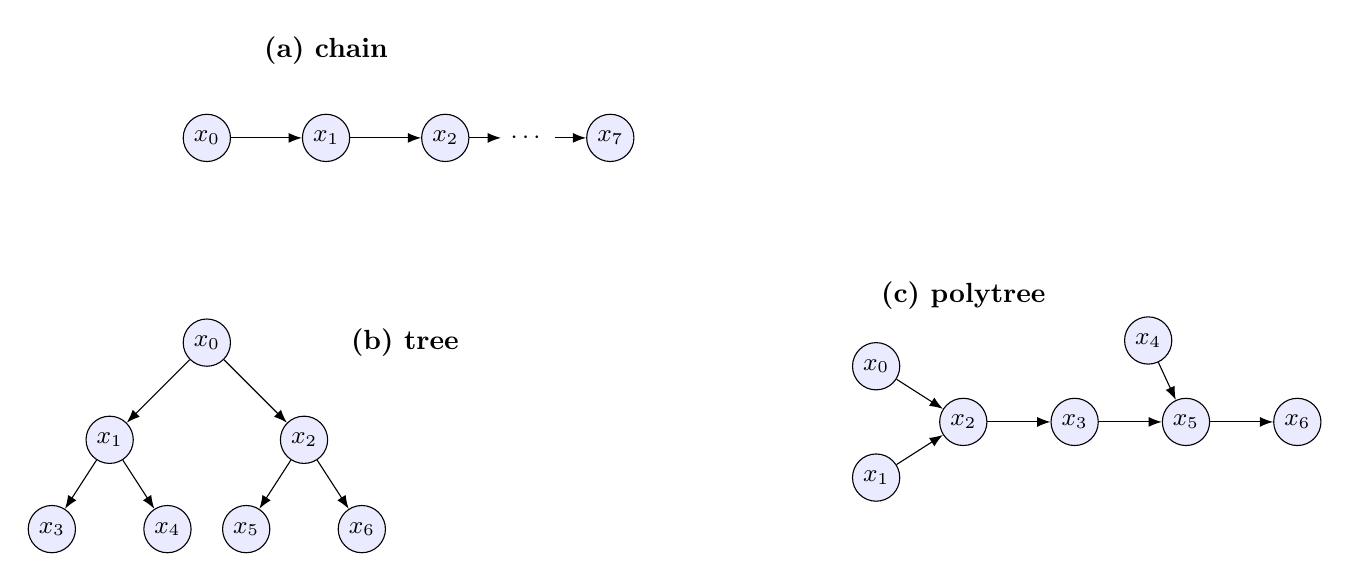
\begin{tikzpicture}[font=\small,>=Latex,node distance=9mm,
  v/.style={circle,draw,fill=blue!8,minimum size=6mm,inner sep=1pt}]
% chain
\begin{scope}
  \node[v](c0){$x_0$}; \node[v,right=of c0](c1){$x_1$};
  \node[v,right=of c1](c2){$x_2$}; \node[right=4mm of c2](cd){$\cdots$};
  \node[v,right=4mm of cd](c7){$x_7$};
  \draw[->](c0)--(c1); \draw[->](c1)--(c2); \draw[->](c2)--(cd); \draw[->](cd)--(c7);
  \node[above=5mm of c1,font=\bfseries]{(a) chain};
\end{scope}
% tree
\begin{scope}[yshift=-2.6cm]
  \node[v](t0){$x_0$};
  \node[v,below left=8mm and 8mm of t0](t1){$x_1$};
  \node[v,below right=8mm and 8mm of t0](t2){$x_2$};
  \node[v,below left=7mm and 3mm of t1](t3){$x_3$};
  \node[v,below right=7mm and 3mm of t1](t4){$x_4$};
  \node[v,below left=7mm and 3mm of t2](t5){$x_5$};
  \node[v,below right=7mm and 3mm of t2](t6){$x_6$};
  \draw[->](t0)--(t1);\draw[->](t0)--(t2);\draw[->](t1)--(t3);\draw[->](t1)--(t4);
  \draw[->](t2)--(t5);\draw[->](t2)--(t6);
  \node[right=14mm of t0,font=\bfseries]{(b) tree};
\end{scope}
% polytree
\begin{scope}[yshift=-2.9cm,xshift=8.5cm]
  \node[v](p0){$x_0$}; \node[v,below=8mm of p0](p1){$x_1$};
  \node[v,right=8mm of $(p0)!0.5!(p1)$](p2){$x_2$};
  \node[v,right=8mm of p2](p3){$x_3$};
  \node[v,right=8mm of p3](p5){$x_5$};
  \node[v,above right=6mm and 5mm of p3](p4){$x_4$};
  \node[v,right=8mm of p5](p6){$x_6$};
  \draw[->](p0)--(p2);\draw[->](p1)--(p2);\draw[->](p2)--(p3);
  \draw[->](p3)--(p5);\draw[->](p4)--(p5);\draw[->](p5)--(p6);
  \node[above=10mm of p2,font=\bfseries]{(c) polytree};
\end{scope}
\end{tikzpicture}
\caption{The three singly-connected \emph{primal} graphs. (a) the Markov chain
  \texttt{chain.lcn} ($n{=}8$); (b) the branching binary tree \texttt{tree.lcn} ($n{=}7$, every
  node has one parent); (c) the polytree \texttt{polytree.lcn} ($n{=}7$) with two colliders
  $x_0,x_1\!\to\!x_2$ and $x_3,x_4\!\to\!x_5$ (multi-parent nodes).}
\label{fig:structures}
\end{figure}

All three have only family-local sentences (a prior on each root and
$P(\text{child}\mid\text{parents})$ on each edge), so the only cross-family constraints are the LMC
independencies, and every structure is singly connected. By Theorem~1, ARIEL should be exact on all
three.

\paragraph{Ground truth.} We compare against two independent exact references:
\texttt{CredalJT} (the junction-tree exact NLP, scheme D5 of the companion note), provably exact on
these structures; and an LMC-correct \emph{brute-force} oracle that optimizes over a parametric
family which satisfies every LMC equality \eqref{eq:lmc} \emph{by construction} (residual
$\sim\!10^{-16}$), using SLSQP only --- hence immune to the nonconvex-solver unreliability that
afflicts \texttt{ExactInference}/SCIP on these bilinear systems. The two references agree to four
decimals on every atom, so we report one ``exact'' column.

\section{ARIEL is exact on all three structures}\label{sec:singly}

Running \texttt{ArielInference.run} (\texttt{n\_iters}$=60$, threshold $10^{-9}$, fully converged)
reproduces the exact marginal bounds on the chain, the tree, and the polytree
(Table~\ref{tab:fixed}) --- to four decimals on every atom, matching both the \texttt{CredalJT} and
the brute-force oracle. This is exactly what Theorem~1 predicts.

\begin{table}[ht]\centering\small
\begin{tabular}{llcc}
\toprule
structure & atom & ARIEL & exact \\
\midrule
\texttt{chain}    & $x_0$ & $[0.3000,0.5000]$ & $[0.3000,0.5000]$ \\
                  & $x_1$ & $[0.4000,0.6800]$ & $[0.4000,0.6800]$ \\
                  & $x_2$ & $[0.3280,0.6400]$ & $[0.3280,0.6400]$ \\
                  & $x_7$ & $[0.3336,0.6667]$ & $[0.3340,0.6670]$ \\
\midrule
\texttt{tree}     & $x_0$ & $[0.3000,0.5000]$ & $[0.3000,0.5000]$ \\
                  & $x_1$ & $[0.4000,0.6800]$ & $[0.4000,0.6800]$ \\
                  & $x_3$ & $[0.3280,0.6400]$ & $[0.3280,0.6400]$ \\
                  & $x_6$ & $[0.3280,0.6400]$ & $[0.3280,0.6400]$ \\
\midrule
\texttt{polytree} & $x_2$ & $[0.3100,0.6300]$ & $[0.3100,0.6300]$ \\
                  & $x_3$ & $[0.3480,0.6760]$ & $[0.3480,0.6760]$ \\
                  & $x_5$ & $[0.2644,0.6528]$ & $[0.2644,0.6528]$ \\
                  & $x_6$ & $[0.3389,0.6942]$ & $[0.3389,0.6942]$ \\
\bottomrule
\end{tabular}
\caption{ARIEL reproduces the exact marginal bounds on all three singly-connected structures
  (residual differences are solver tolerance, $\le 4\times10^{-4}$), confirming Theorem~1. Bounds
  are stable from $10$ iterations onward.}
\label{tab:fixed}
\end{table}

\section{The factor graph of the tree, and its bipartite tree shape}\label{sec:treefg}

To analyse \emph{why} exactness holds we need the factor graph itself, not just the primal graph.
For the tree of Figure~\ref{fig:structures}(b), the sentences group by scope into seven factors:
\[
  f_1{=}\{x_0,x_1\},\ f_2{=}\{x_0,x_2\},\ f_3{=}\{x_1,x_3\},\ f_4{=}\{x_1,x_4\},\
  f_5{=}\{x_2,x_5\},\ f_6{=}\{x_2,x_6\},\ f_7{=}\{x_0\},
\]
where $f_7$ holds the root prior $P(x_0)$ and each $f_i$ ($i\le 6$) holds the two transition
sentences $P(\text{child}\mid\text{parent}),P(\text{child}\mid\neg\text{parent})$ of one tree edge.
Figure~\ref{fig:treefg} draws the bipartite factor graph. \textbf{It is itself a tree}: there is no
cycle through variable and factor nodes. This is the property Theorem~1 hinges on.

\begin{figure}[ht]
\centering
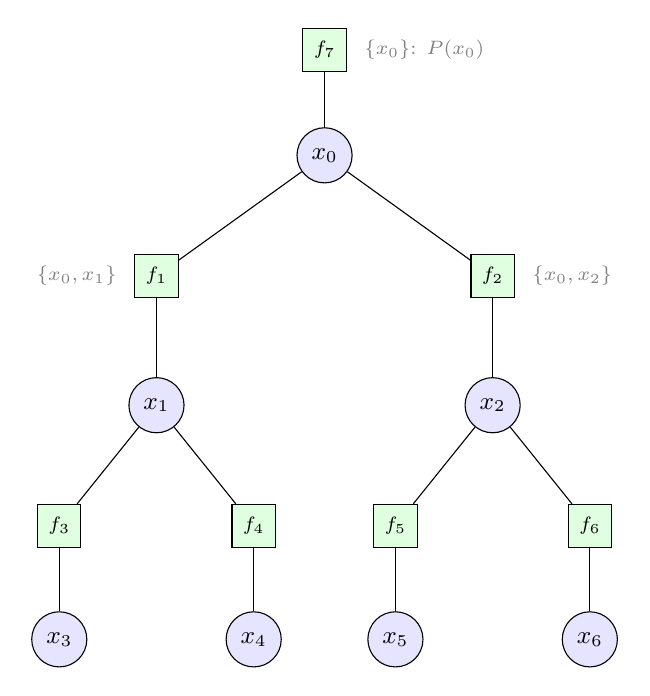
\begin{tikzpicture}[font=\small,>=Latex,
  v/.style={circle,draw,fill=blue!10,minimum size=7mm,inner sep=1pt},
  f/.style={rectangle,draw,fill=green!12,minimum size=5.5mm,inner sep=2pt,font=\scriptsize}]
% variable nodes (the tree layout)
\node[v](x0){$x_0$};
\node[f,above=7mm of x0](f7){$f_7$};
\node[f,below left=10mm and 16mm of x0](f1){$f_1$};
\node[f,below right=10mm and 16mm of x0](f2){$f_2$};
\node[v,below=10mm of f1](x1){$x_1$};
\node[v,below=10mm of f2](x2){$x_2$};
\node[f,below left=10mm and 7mm of x1](f3){$f_3$};
\node[f,below right=10mm and 7mm of x1](f4){$f_4$};
\node[f,below left=10mm and 7mm of x2](f5){$f_5$};
\node[f,below right=10mm and 7mm of x2](f6){$f_6$};
\node[v,below=8mm of f3](x3){$x_3$};
\node[v,below=8mm of f4](x4){$x_4$};
\node[v,below=8mm of f5](x5){$x_5$};
\node[v,below=8mm of f6](x6){$x_6$};
% edges
\draw(x0)--(f7);
\draw(x0)--(f1);\draw(f1)--(x1);
\draw(x0)--(f2);\draw(f2)--(x2);
\draw(x1)--(f3);\draw(f3)--(x3);
\draw(x1)--(f4);\draw(f4)--(x4);
\draw(x2)--(f5);\draw(f5)--(x5);
\draw(x2)--(f6);\draw(f6)--(x6);
% scope annotations
\node[right=1mm of f7,font=\scriptsize,gray]{$\{x_0\}$: $P(x_0)$};
\node[left=1mm of f1,font=\scriptsize,gray]{$\{x_0,x_1\}$};
\node[right=1mm of f2,font=\scriptsize,gray]{$\{x_0,x_2\}$};
\end{tikzpicture}
\caption{The bipartite \emph{factor graph} of \texttt{tree.lcn}: circles are variable nodes
  (atoms), squares are factor nodes. $f_7=\{x_0\}$ carries the root prior; each $f_i$ ($i\le6$)
  carries the two transition sentences of one tree edge. Crucially the bipartite graph is a
  \emph{tree} --- removing any factor disconnects the graph, and any two variables communicate
  along a unique factor path. This is what makes the interval-message summary lossless
  (Section~\ref{sec:lmcpreserve}).}
\label{fig:treefg}
\end{figure}

The chain's factor graph is the special case where the tree is a path: factors
$f_i=\{x_{i-1},x_i\}$ in a line plus the prior $\{x_0\}$. The polytree's factor graph is also a
tree, but with two $3$-atom factors at the colliders:
$\{x_0,x_1,x_2\}$, $\{x_3,x_4,x_5\}$, joined by $\{x_2,x_3\}$ and $\{x_5,x_6\}$ and the root priors
$\{x_0\},\{x_1\},\{x_4\}$. In all three cases the factor graph is singly connected.

\section{How the factor graph preserves the LMC}\label{sec:lmcpreserve}

This is the crux. ARIEL never builds the global $2^n$ joint, so it cannot impose the LMC equalities
\eqref{eq:lmc} globally. There are exactly two ways an LMC assertion can survive into ARIEL's
answer: it can be \textbf{imposed} (its full scope $x\cup Y\cup S$ fits inside one factor, so
\eqref{eq:lmc} is added to that factor's local NLP, step (ii) of Section~\ref{sec:bg}), or it can be
\textbf{preserved structurally} (the factor-graph topology and the message protocol already entail
it). We examine which happens.

\subsection{On the test structures, every LMC is dropped --- yet exactness holds}
Table~\ref{tab:lmc} runs the contrast (\texttt{ArielInference.analyze}) for the three structures.
The striking fact: \emph{on all three, not one LMC assertion fits inside a single factor}, so
\emph{none is imposed} as an explicit constraint. The local NLPs contain only sentence rows and
neighbour intervals --- no LMC equalities at all.

\begin{table}[ht]\centering\small
\begin{tabular}{lccp{6.2cm}}
\toprule
structure & \#LMC assertions & \#imposed (fit a factor) & why every LMC spans $\ge2$ factors \\
\midrule
\texttt{chain}    & 6 & 0 & e.g.\ $(x_2\indep x_0\mid x_1)$ has scope $\{x_0,x_1,x_2\}$; factors are $2$-atom edges, so $x_0,x_2$ never co-occur \\
\texttt{tree}     & 6 & 0 & e.g.\ $(x_1\indep x_2,x_5,x_6\mid x_0)$ spans the whole left/right subtrees \\
\texttt{polytree} & 7 & 0 & e.g.\ $(x_0\indep x_1,x_4)$ has scope $\{x_0,x_1,x_4\}$ straddling \emph{both} collider factors \\
\bottomrule
\end{tabular}
\caption{On the chain, tree and polytree, \emph{no} LMC assertion fits inside a single factor, so
  \emph{none} is imposed as an explicit equality in any local NLP. Despite this, ARIEL is exact
  (Table~\ref{tab:fixed}). The LMC must therefore be preserved \emph{structurally}.}
\label{tab:lmc}
\end{table}

So the LMC equalities are \emph{not} enforced anywhere as constraints, yet the bounds are exact.
The resolution is that on a singly-connected factor graph the message protocol \emph{is} the LMC.

\subsection{Why the interval summary is exactly the LMC factorization}
Consider a factor $f$ with target $n$ and one other boundary variable $m$ (the chain/tree case).
When ARIEL computes $f\!\to\!n$, the variable $m$ enters the local NLP only through its marginal
interval. Equivalently, $f$ treats $m$ as \emph{independent of everything reached through $m$'s
other factors, given the value summarized by the interval}. On the tree of
Figure~\ref{fig:treefg}, $m$ is precisely a \emph{separator}: deleting $m$ from the factor tree
disconnects $f$'s side from the rest. The variables on the far side of $m$ are LMC-independent of
$n$ given $m$ --- that is exactly assertion \eqref{eq:lmc} with $S=\{m\}$. Thus
\begin{quote}\emph{the interval message across a separator $m$ encodes the LMC independence
``everything on $f$'s side $\indep$ everything beyond $m$ $\mid m$'' --- the very assertion that was
``dropped''.} \end{quote}
Because the factor graph is a tree, every LMC assertion decomposes into such single-separator
statements along the unique path between the relevant variables, and each is realized by one
interval message. No global joint, and no explicit equality, is needed: the topology supplies the
factorization. This is the LCN analogue of why sum-product belief propagation is exact on trees.

\subsection{The collider case: the LMC lives \emph{inside} a factor's joint}
The polytree is more subtle because moralizing a collider $x_0,x_1\!\to\!x_2$ puts all three atoms
in one factor $\{x_0,x_1,x_2\}$ (its sentences are $P(x_2\mid x_0,x_1)$, which mention all three).
The relevant LMC here is the \emph{co-parent} independence $(x_0\indep x_1)$. Two observations make
this exact:
\begin{enumerate}
  \item \textbf{Inside the factor, the full $2^3$ joint is modelled}, so the collider conditional
    $P(x_2\mid x_0,x_1)$ is represented exactly --- nothing about the $x_0$--$x_1$--$x_2$
    interaction is approximated within $f$.
  \item \textbf{The co-parent independence $(x_0\indep x_1)$ is \emph{not} imposed} (its scope
    $\{x_0,x_1\}$ does fit the factor, but the assertion the LMC actually generates is
    $(x_0\indep x_1,x_4)$, scope $\{x_0,x_1,x_4\}$, which spans both colliders --- Table~\ref{tab:lmc}).
    It does not need to be: the only messages \emph{leaving} the collider factor go to $x_2$
    (toward the rest of the chain) and back to the priors $x_0,x_1$; along the factor tree, $x_0$
    and $x_1$ have no second path to influence each other, so leaving them free inside $f$ cannot
    create spurious correlation in any marginal. The brute-force oracle confirms the resulting
    $P(x_2),P(x_3),\dots$ are exact (Table~\ref{tab:fixed}).
\end{enumerate}
Indeed ARIEL's outgoing messages \emph{implicitly assert} pairwise independencies among a factor's
boundary that are \emph{not} in the LMC --- for the collider factor these include the (false)
$(x_0\indep x_2)$ and $(x_1\indep x_2)$ (\texttt{analyze} reports them under ``added by ARIEL, not
in LMC''). These are harmless on a tree precisely because they only ever summarize a message along
a single factor path; there is no returning path on which the missing correlation could matter.

\subsection{When an LMC \emph{does} fit a factor it \emph{is} imposed}
The structural mechanism above is not the whole story --- step (ii) of Section~\ref{sec:bg} is live.
When an LMC assertion's full scope happens to fit one factor, ARIEL adds its equality
\eqref{eq:lmc} to that factor's local NLP. For instance on \texttt{asia} the assertion
$(C\indep B\mid S)$ has scope $\{B,C,S\}$, which equals the factor $\{B,C,S\}$, and \texttt{analyze}
reports it as \emph{enforced} (while the three wider asia assertions are dropped/structural).
So ARIEL's LMC handling is two-tier: \textbf{impose where the scope fits a factor; rely on the
factor tree elsewhere}. On a singly-connected graph the second tier is exact; the first tier is a
bonus that tightens factors with $\ge3$ atoms.

\subsection{Summary of LMC preservation}
\begin{proposition}[LMC preservation on singly-connected factor graphs]\label{prop:lmc}
Let the factor graph $\mathcal F$ be singly connected (a tree). Then for every LMC assertion
$(x\indep Y\mid S)$:
\begin{itemize}
  \item if $x\cup Y\cup S\subseteq\mathrm{scope}(f)$ for some factor $f$, the equality
    \eqref{eq:lmc} is imposed in $f$'s local NLP (exact, by construction); otherwise
  \item the assertion factorizes into single-separator independencies along the unique factor path
    connecting $x$, $Y$ and $S$, each of which is realized exactly by an interval message across
    that separator.
\end{itemize}
In both cases the assertion holds in ARIEL's converged solution, so the bounds equal the exact LCN
bounds (Table~\ref{tab:fixed}). The interval summary is information-lossless precisely because a
tree has no second path along which a discarded joint correlation could matter.
\end{proposition}

\section{The boundary: a loopy instance where the LMC is no longer preserved}\label{sec:loopy}

Proposition~\ref{prop:lmc} fails the moment the factor graph has a cycle, because then a separator
no longer disconnects the graph and the interval summary drops correlation that a \emph{second}
path needs. We exhibit this with the \textbf{diamond} $A\!\to\!\{B,C\}$, $\{B,C\}\!\to\!D$ (collider
at $D$) plus a single \emph{cross-family} sentence coupling the co-parents:
\[
  P(A)\!\in\![0.4,0.6],\quad P(B\mid A),P(C\mid A),\quad P(D\mid B,C)\ (\text{4 rows}),\quad
  \boxed{P(B\land C)\le 0.25}.
\]
The skeleton has the $4$-cycle $A\!-\!B\!-\!D\!-\!C\!-\!A$ and the extra sentence
$P(B\land C)$ adds a second loop, so the factor graph is \emph{loopy} ($2$ independent cycles); the
instance is consistent. Table~\ref{tab:loopy} compares ARIEL with the exact bounds (confirmed by
both \texttt{CredalJT} and the brute-force oracle, LMC residual $2\times10^{-16}$).

\begin{table}[ht]\centering\small
\begin{tabular}{lccc}
\toprule
atom & ARIEL & exact & verdict \\
\midrule
$A$ & $[0.4000,0.6000]$ & $[0.4000,0.6000]$ & exact \\
$B$ & $[0.3600,\mathbf{0.6400}]$ & $[0.3600,\mathbf{0.5700}]$ & \emph{outer} ($+0.07$) \\
$C$ & $[0.3600,\mathbf{0.6400}]$ & $[0.3600,\mathbf{0.5700}]$ & \emph{outer} ($+0.07$) \\
$D$ & $[0.3160,\mathbf{0.6840}]$ & $[0.3160,\mathbf{0.5940}]$ & \emph{outer} ($+0.09$) \\
\bottomrule
\end{tabular}
\caption{On the loopy coupled diamond, ARIEL is only a valid \emph{outer} bound: the upper bounds of
  $B$, $C$, $D$ are $0.07$--$0.09$ too high. The cross-family sentence $P(B\land C)\le0.25$ lives in
  the factor $\{B,C\}$, but the messages it sends to $B$ and to $C$ carry only the \emph{marginal}
  intervals $P(B)$, $P(C)$ --- they cannot transmit the \emph{joint} restriction on $B\land C$
  around the loop, so the cap never tightens the rest.}
\label{tab:loopy}
\end{table}

This is the interval-message approximation of Section~\ref{sec:approx} biting: the factor $\{B,C\}$
\emph{knows} $P(B\land C)\le0.25$ but can only \emph{report} marginal intervals on $B$ and $C$ to
the rest of the graph. The joint information is lost at the message boundary --- exactly the failure
mode loopy belief propagation exhibits in classical graphical models. The same mechanism would make
a \emph{spanning} LMC equality non-preservable on a loopy graph: with two paths between two
variables, the single-separator decomposition of Proposition~\ref{prop:lmc} no longer exists.
ARIEL remains \emph{sound} (its interval contains the truth) but not \emph{tight}.

\section{Can ARIEL ever be exact? --- the precise answer}\label{sec:verdict}

\begin{proposition}[What the experiments establish]\label{prop:verdict}
For the marginal task on binary LCNs:
\begin{enumerate}
  \item[\textnormal{(i)}] \textbf{Yes, ARIEL is exact on singly-connected LCNs.} It returns the
    exact posterior marginal bounds on the \texttt{chain}, the branching \texttt{tree}, and the
    \texttt{polytree} (Table~\ref{tab:fixed}), confirming Theorem~1. It is also exact on several
    \emph{loopy} instances whose cycles do not bind (e.g.\ \texttt{cancer}, \texttt{asia},
    \texttt{d4\_biting}, the \emph{un}coupled diamond), but that is incidental, not guaranteed.
  \item[\textnormal{(ii)}] \textbf{Not in general on loopy LCNs.} When a cross-family constraint (or
    a spanning LMC) couples variables that the factor graph can only separate through marginal
    intervals (the coupled diamond, Table~\ref{tab:loopy}), ARIEL is a valid \emph{outer} bound but
    not tight. This is inherent to interval message passing and matches the paper's restriction of
    Theorem~1 to the singly-connected case.
  \item[\textnormal{(iii)}] \textbf{The LMC is preserved without ever being globally imposed.} On
    the test structures \emph{no} LMC fits a single factor (Table~\ref{tab:lmc}); the LMC survives
    structurally, because the bipartite factor graph is a tree and each (dropped) assertion
    decomposes into single-separator independencies realized exactly by the interval messages
    (Proposition~\ref{prop:lmc}). When a scope \emph{does} fit a factor (e.g.\ asia's
    $(C\indep B\mid S)$), the equality is additionally imposed inside that factor's local NLP.
\end{enumerate}
\end{proposition}

\paragraph{Practical takeaway.} ARIEL's exactness on chains, trees and polytrees is real and rests
on a clean principle: \emph{a singly-connected factor graph turns every LMC independence into a
sequence of separator marginals that interval messages transmit losslessly}. The exact moment that
principle breaks is a cycle in the factor graph --- introduced by a cross-family sentence or by a
moralization that leaves two variables with a second communication path --- after which ARIEL is a
sound outer bound rather than an exact one.

\paragraph{Reproducibility.} All numbers come from \texttt{examples/chain.lcn},
\texttt{examples/tree.lcn}, \texttt{examples/polytree.lcn}, and the coupled diamond
($P(B\land C)\le0.25$ added to the four-atom collider). The factor graphs and the LMC contrast are
produced by \texttt{ArielInference.analyze}. The exact references are \texttt{CredalJT}
(\texttt{cn/junction\_nlp.py}, \texttt{solver="scip"}) and an LMC-correct parametric brute-force
oracle (SLSQP).

\end{document}
